\subsection{The Implementation of PID}
\subsubsection{One-axis setup}

Making PID for all axis is possible, but not ideal as determining the source of the problem is more difficult. Therefore, it was decided to tune one axis at a time, excluding the Z-axis which would be tuned after fully calibrating the rest, as it is non-linear.

\begin{figure}[h]
    \centering
    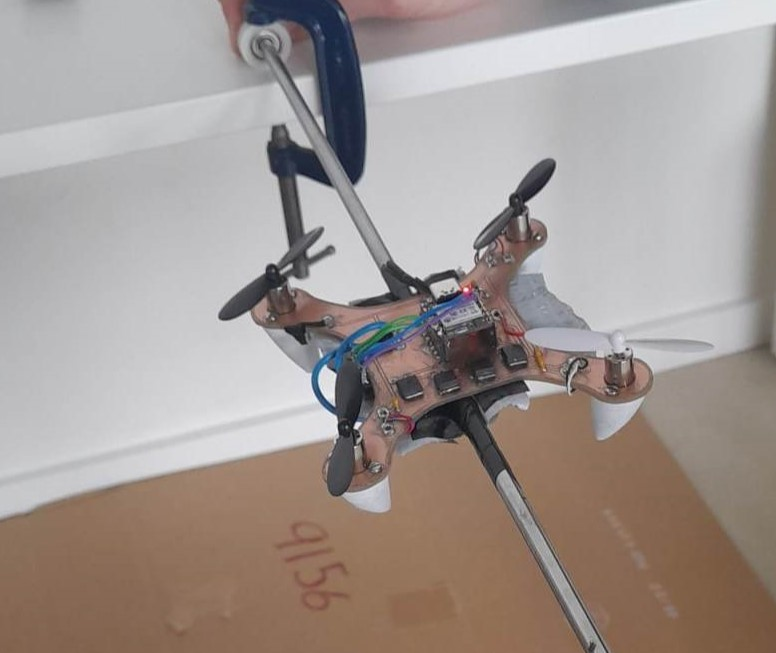
\includegraphics[width=0.5\textwidth]{pictures/Axis_rig.jpg}
    \caption{Picture of axis rig}
    \label{fig:axis_rig}
\end{figure}

The initial 'P' calculation was made from the simulation formula for maximum thrust. The value was calculated to be 0.0045, but as seen in figure \ref{fig:Phi0}, the system is stable, but for the Z-N method, systems need to be marginally stable as shown in figure \ref{fig:Phi1}. 

In figure \ref{fig:Phi0}, the PWM effect of PID on motors is also shown to make sure that QuickPID works as predicted and without delay.
To test the stability of system, it was displaced by a finger in order to mimic large turbulence.

\begin{figure}[h!]
    \centering
    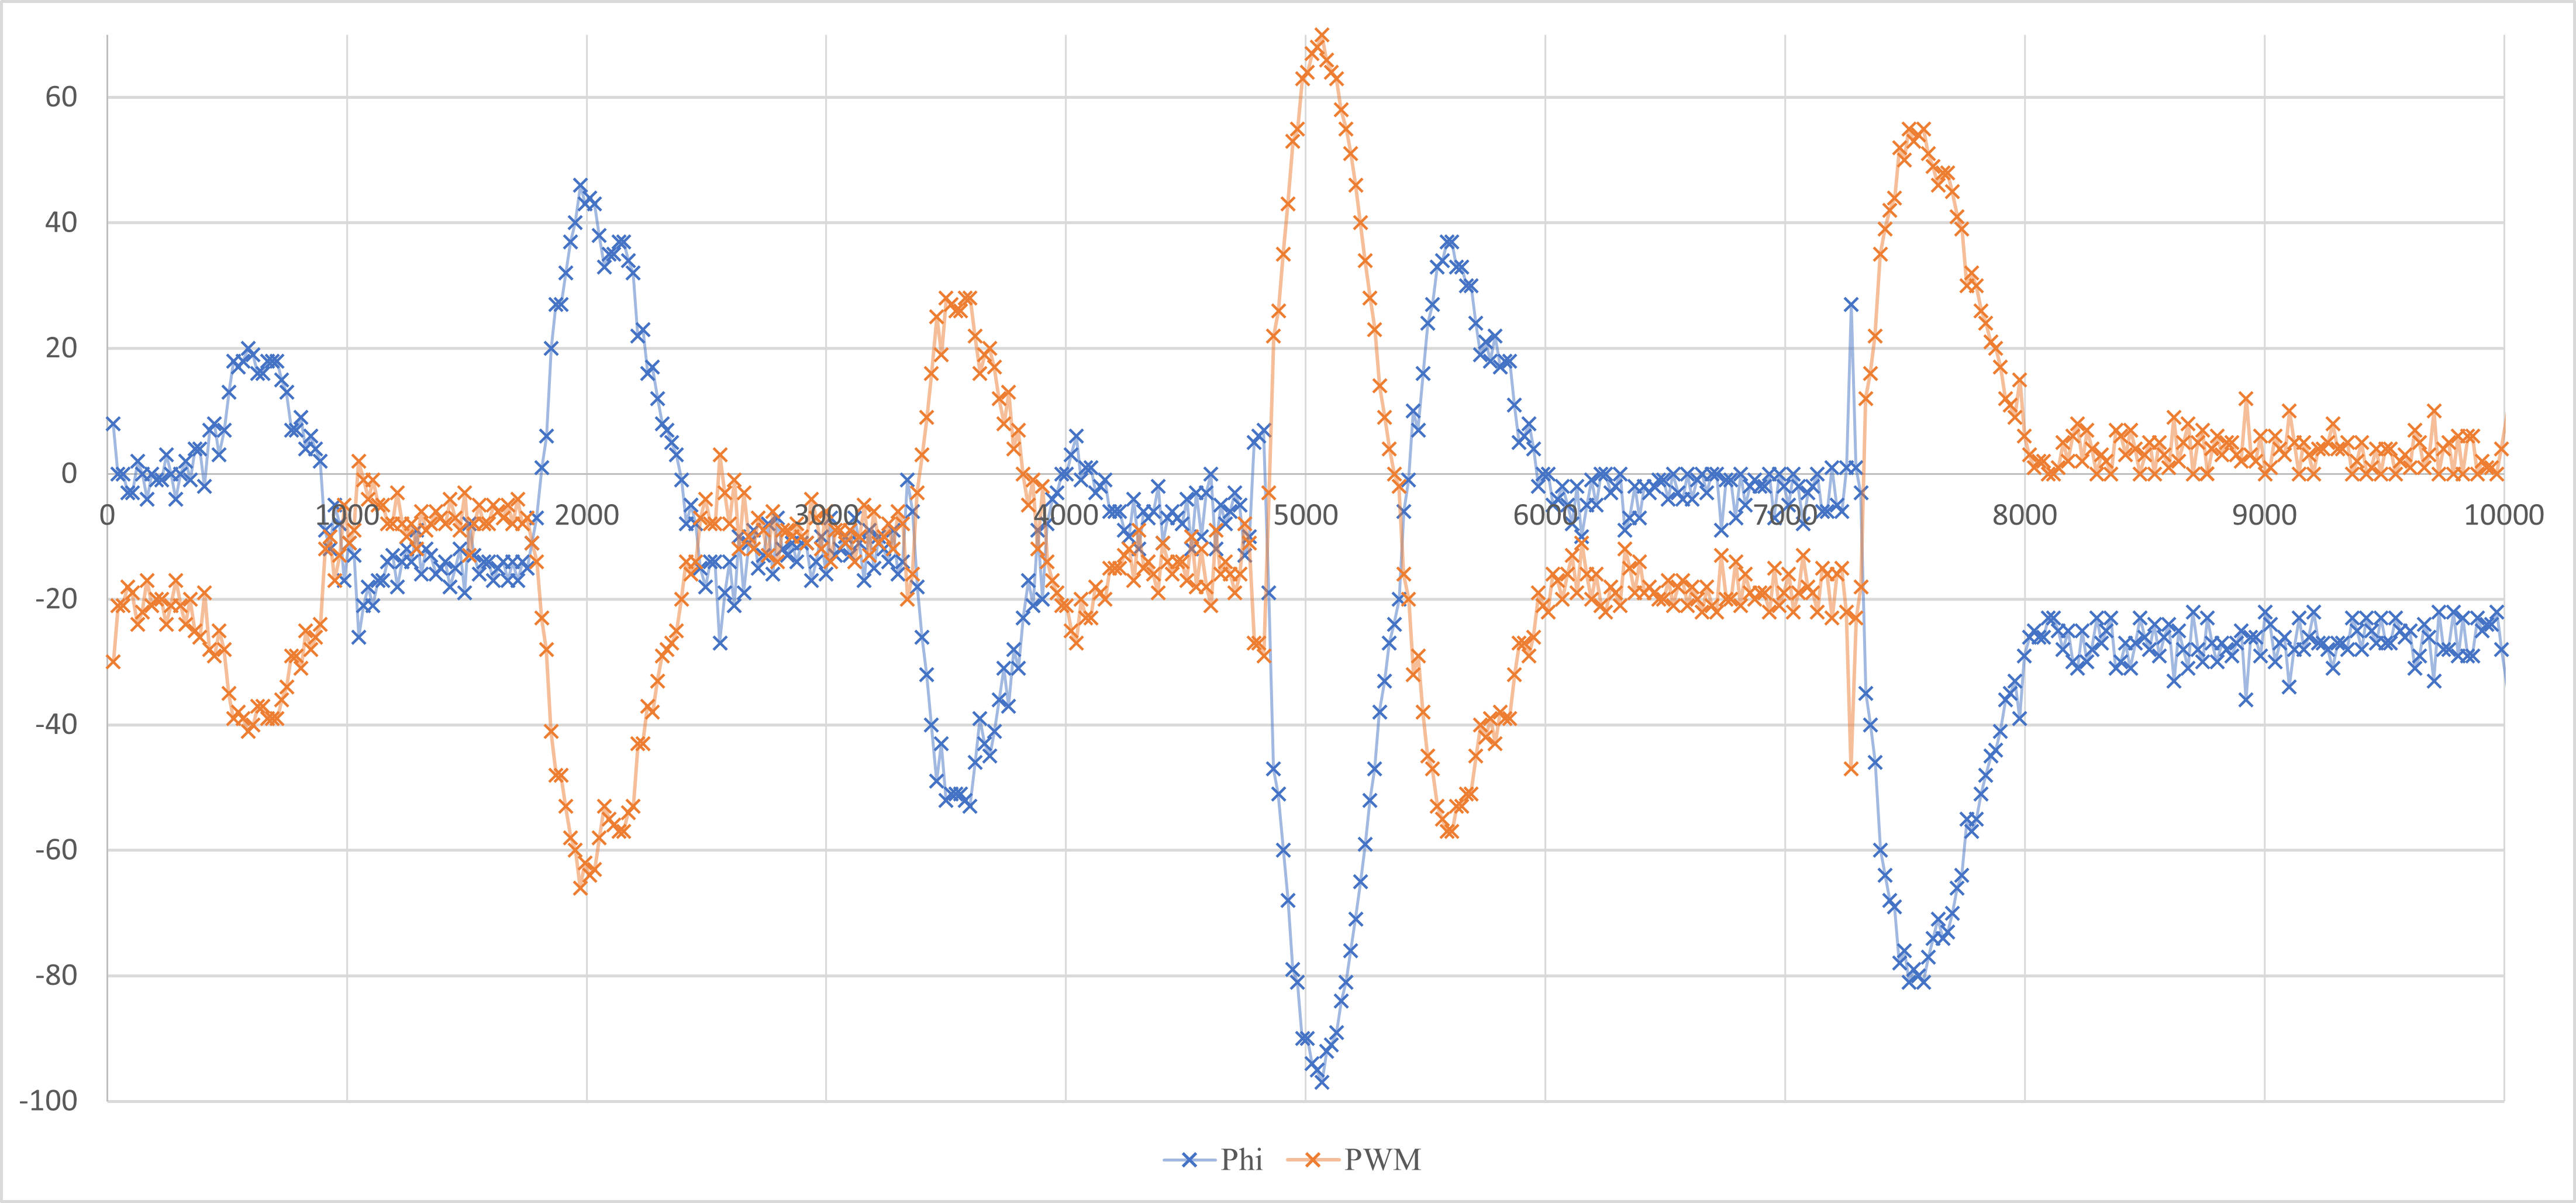
\includegraphics[width=\textwidth]{pictures/graphs/PhiP00045.png}
    \caption{Plot of marginally stable system on Y-axis with purely proportional control}
    \label{fig:Phi0}
\end{figure}

\begin{figure}[h!]
    \centering
    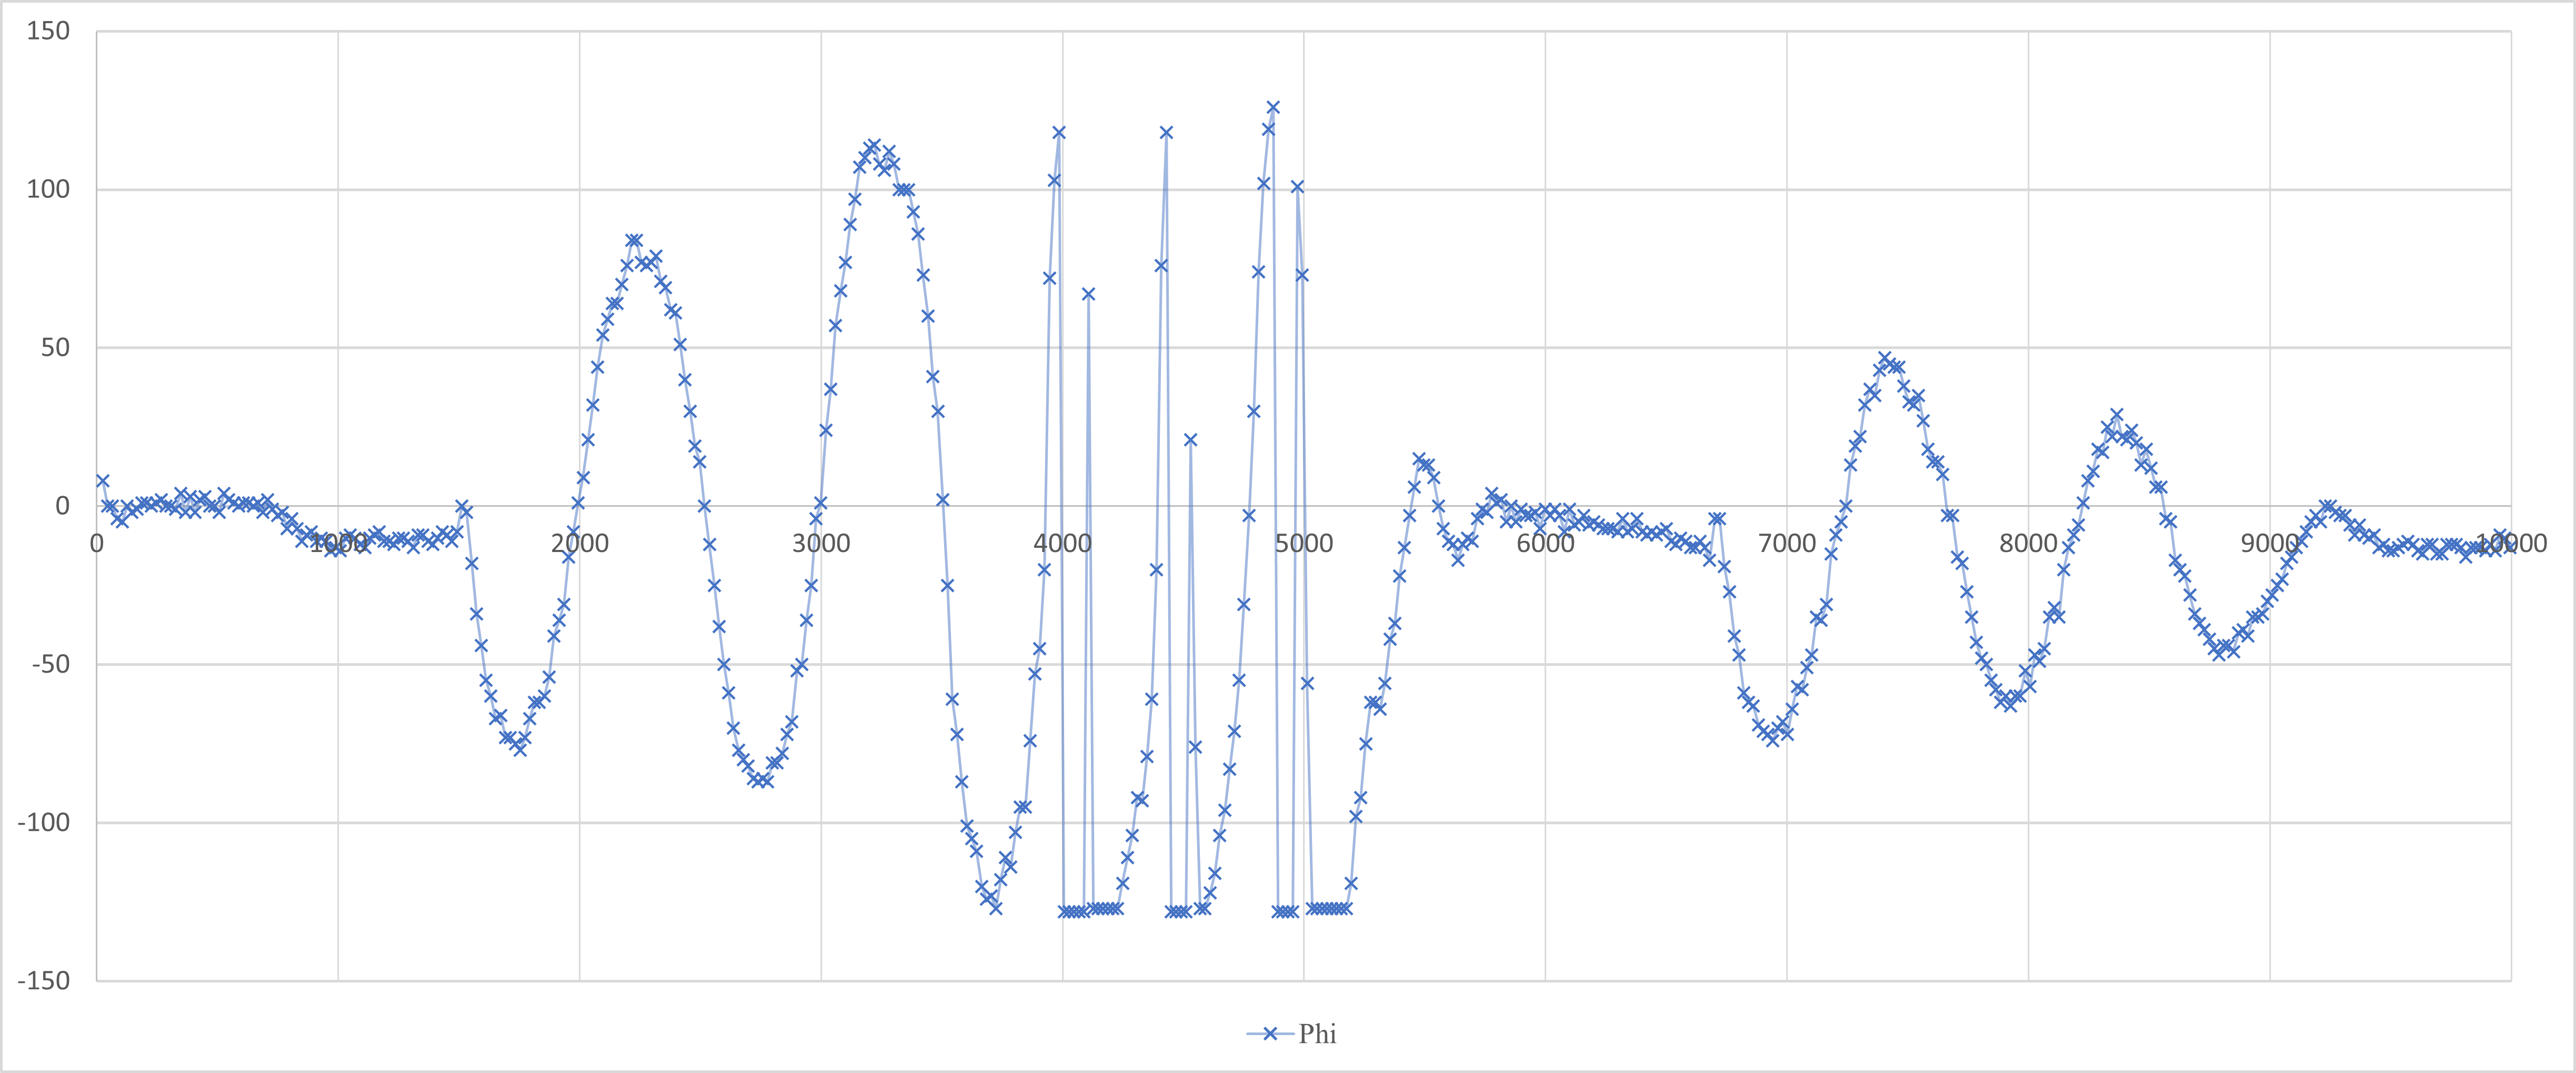
\includegraphics[width=\textwidth]{pictures/graphs/PhiP00065.png}
    \caption{Plot of stable system on Y-axis with purely proportional control}
    \label{fig:Phi1}
\end{figure}

After determining the marginally stable value of P to be 0.0065, the Z-N method was used and applied to the system resulting in figure \ref{fig:PhiZN}. The system is stable, but has a large settling time and long period. This was improved by enlarging the 'P' constant by 0.002 as shown in figure \ref{fig:PhiZN_cal}.

\begin{figure}[h!]
    \centering
    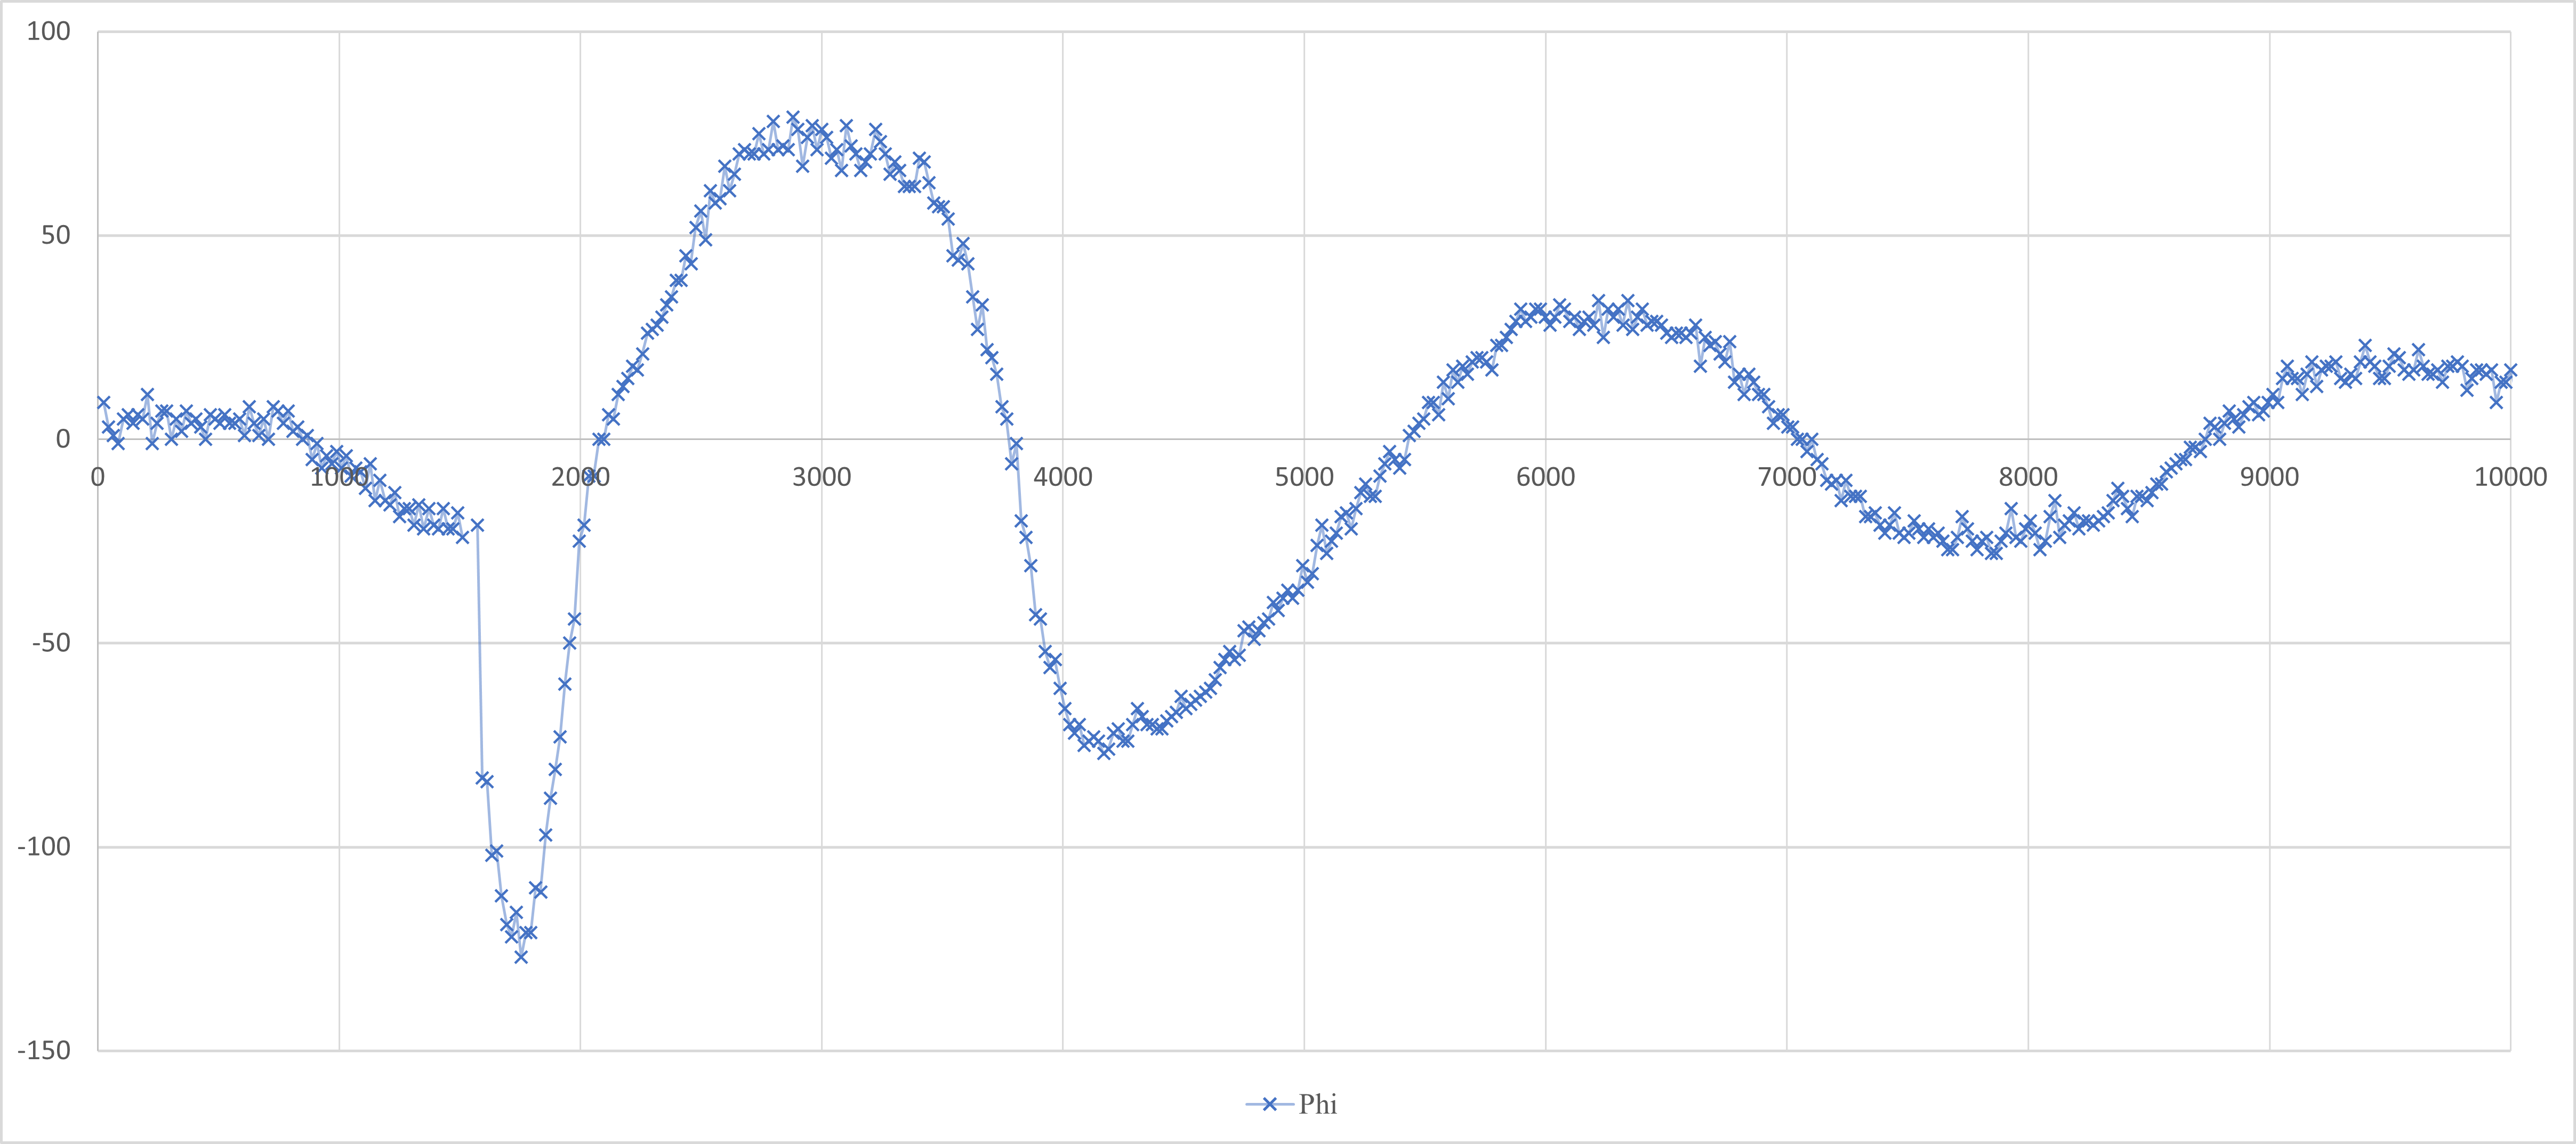
\includegraphics[width=\textwidth]{pictures/graphs/PhiZN.png}
    \caption{Plot of the drone on Y-axis with values from Z-N method}
    \label{fig:PhiZN}
\end{figure}

\begin{figure}[h!]
    \centering
    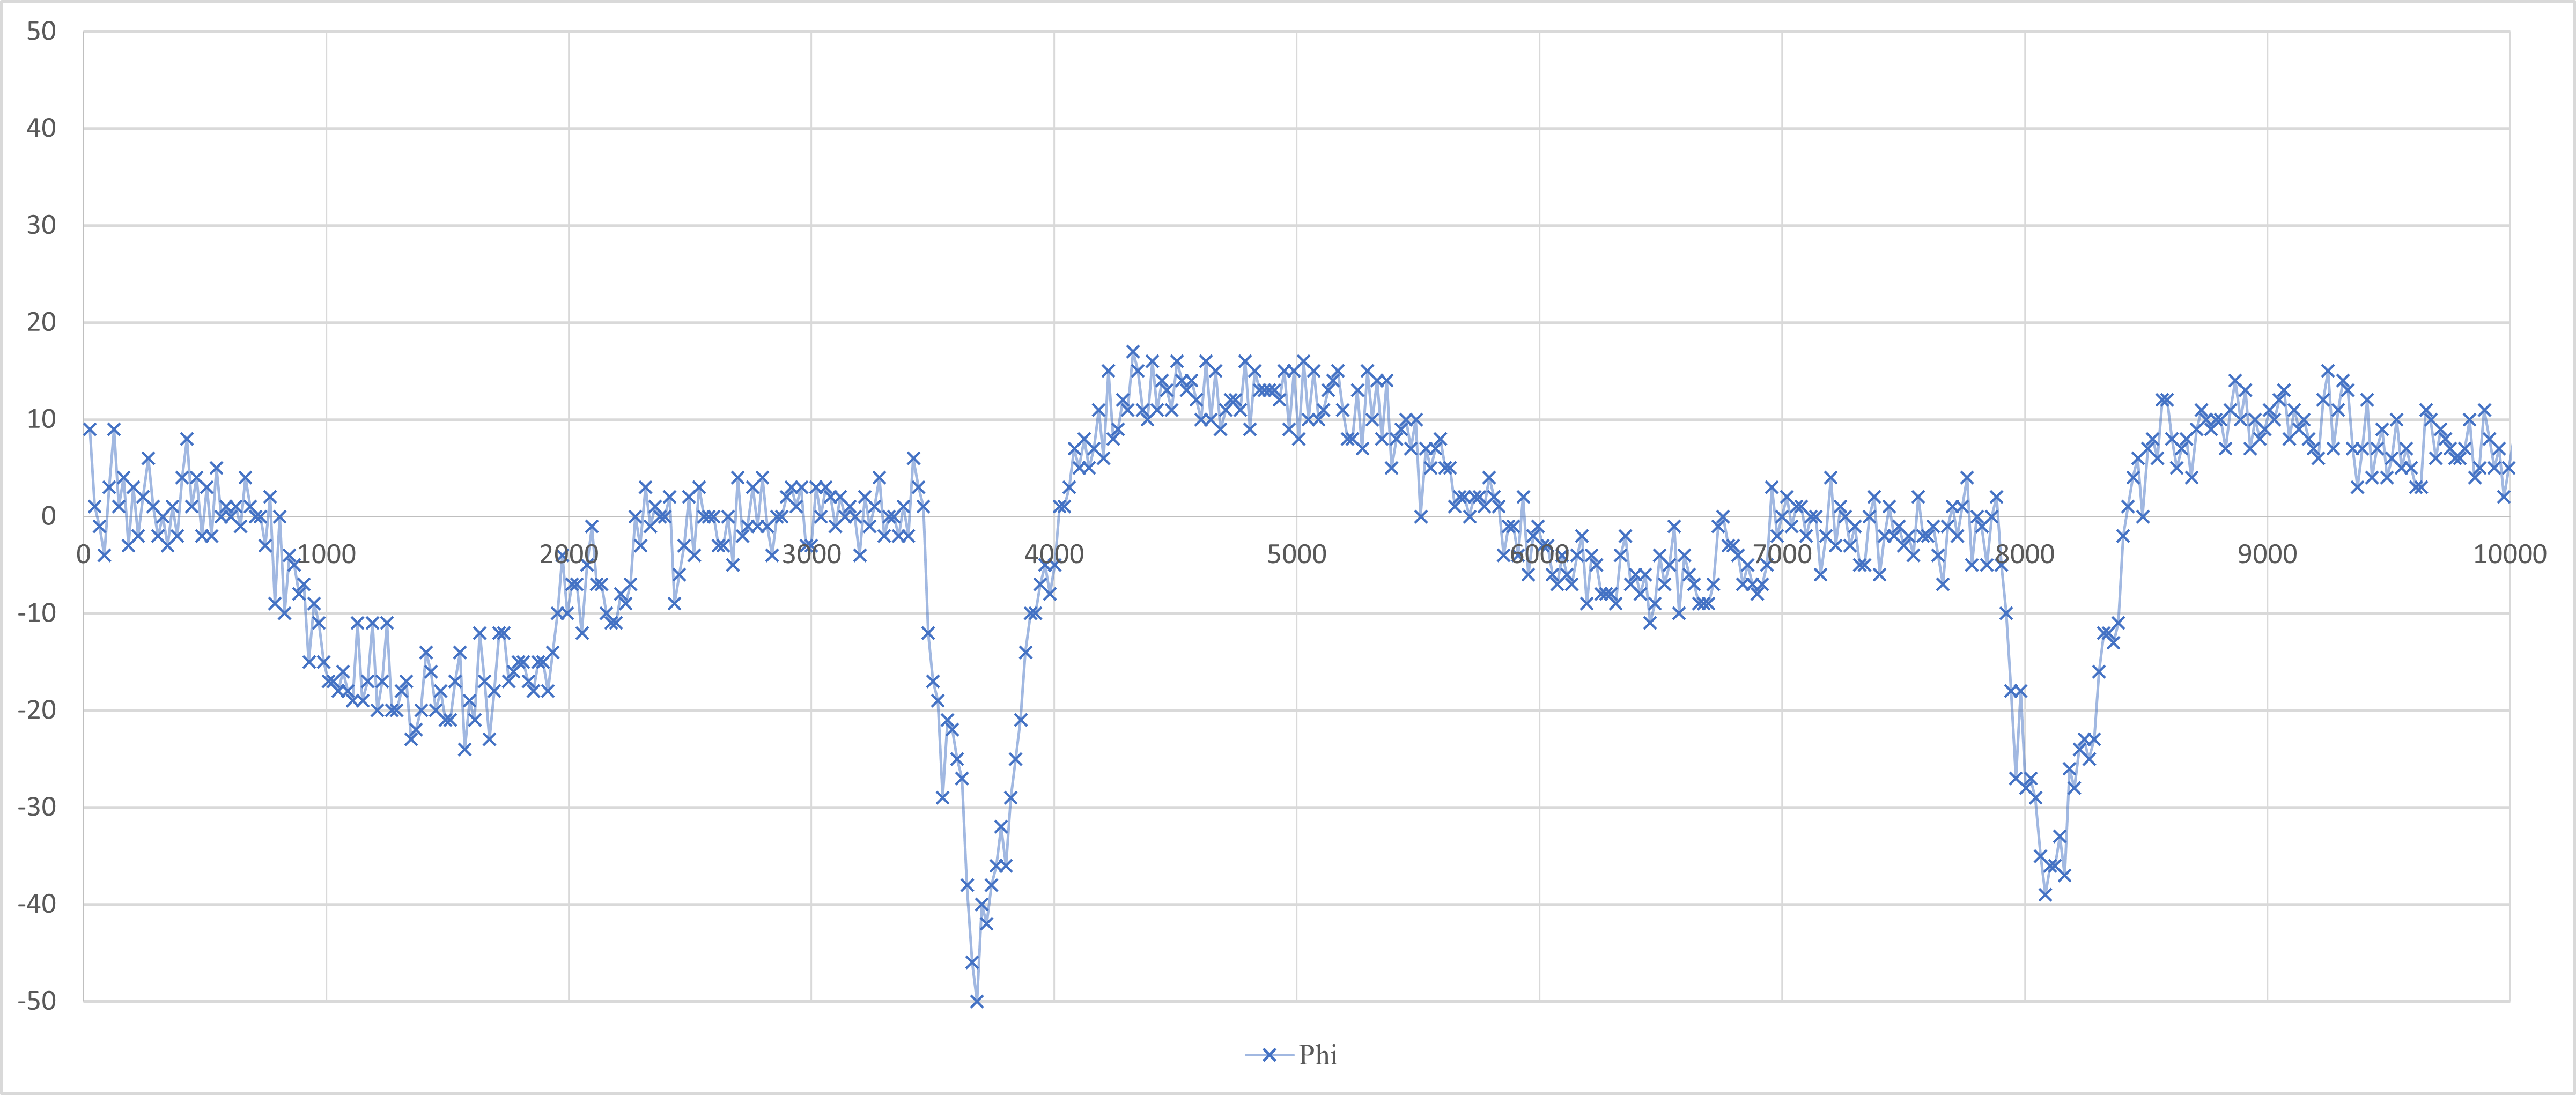
\includegraphics[width=\textwidth]{pictures/graphs/PhiZN_cal.png}
    \caption{Plot of the drone on Y-axis with calibrated values from Z-N method}
    \label{fig:PhiZN_cal}
\end{figure}

For tuning the $\theta$, the same testing rig was utilised and the values of the calibrated $\phi$ were used as starting point. Those were calibrated and the result is shown in figure \ref{fig:Theta_ZN}.

\begin{figure}[h!]
    \centering
    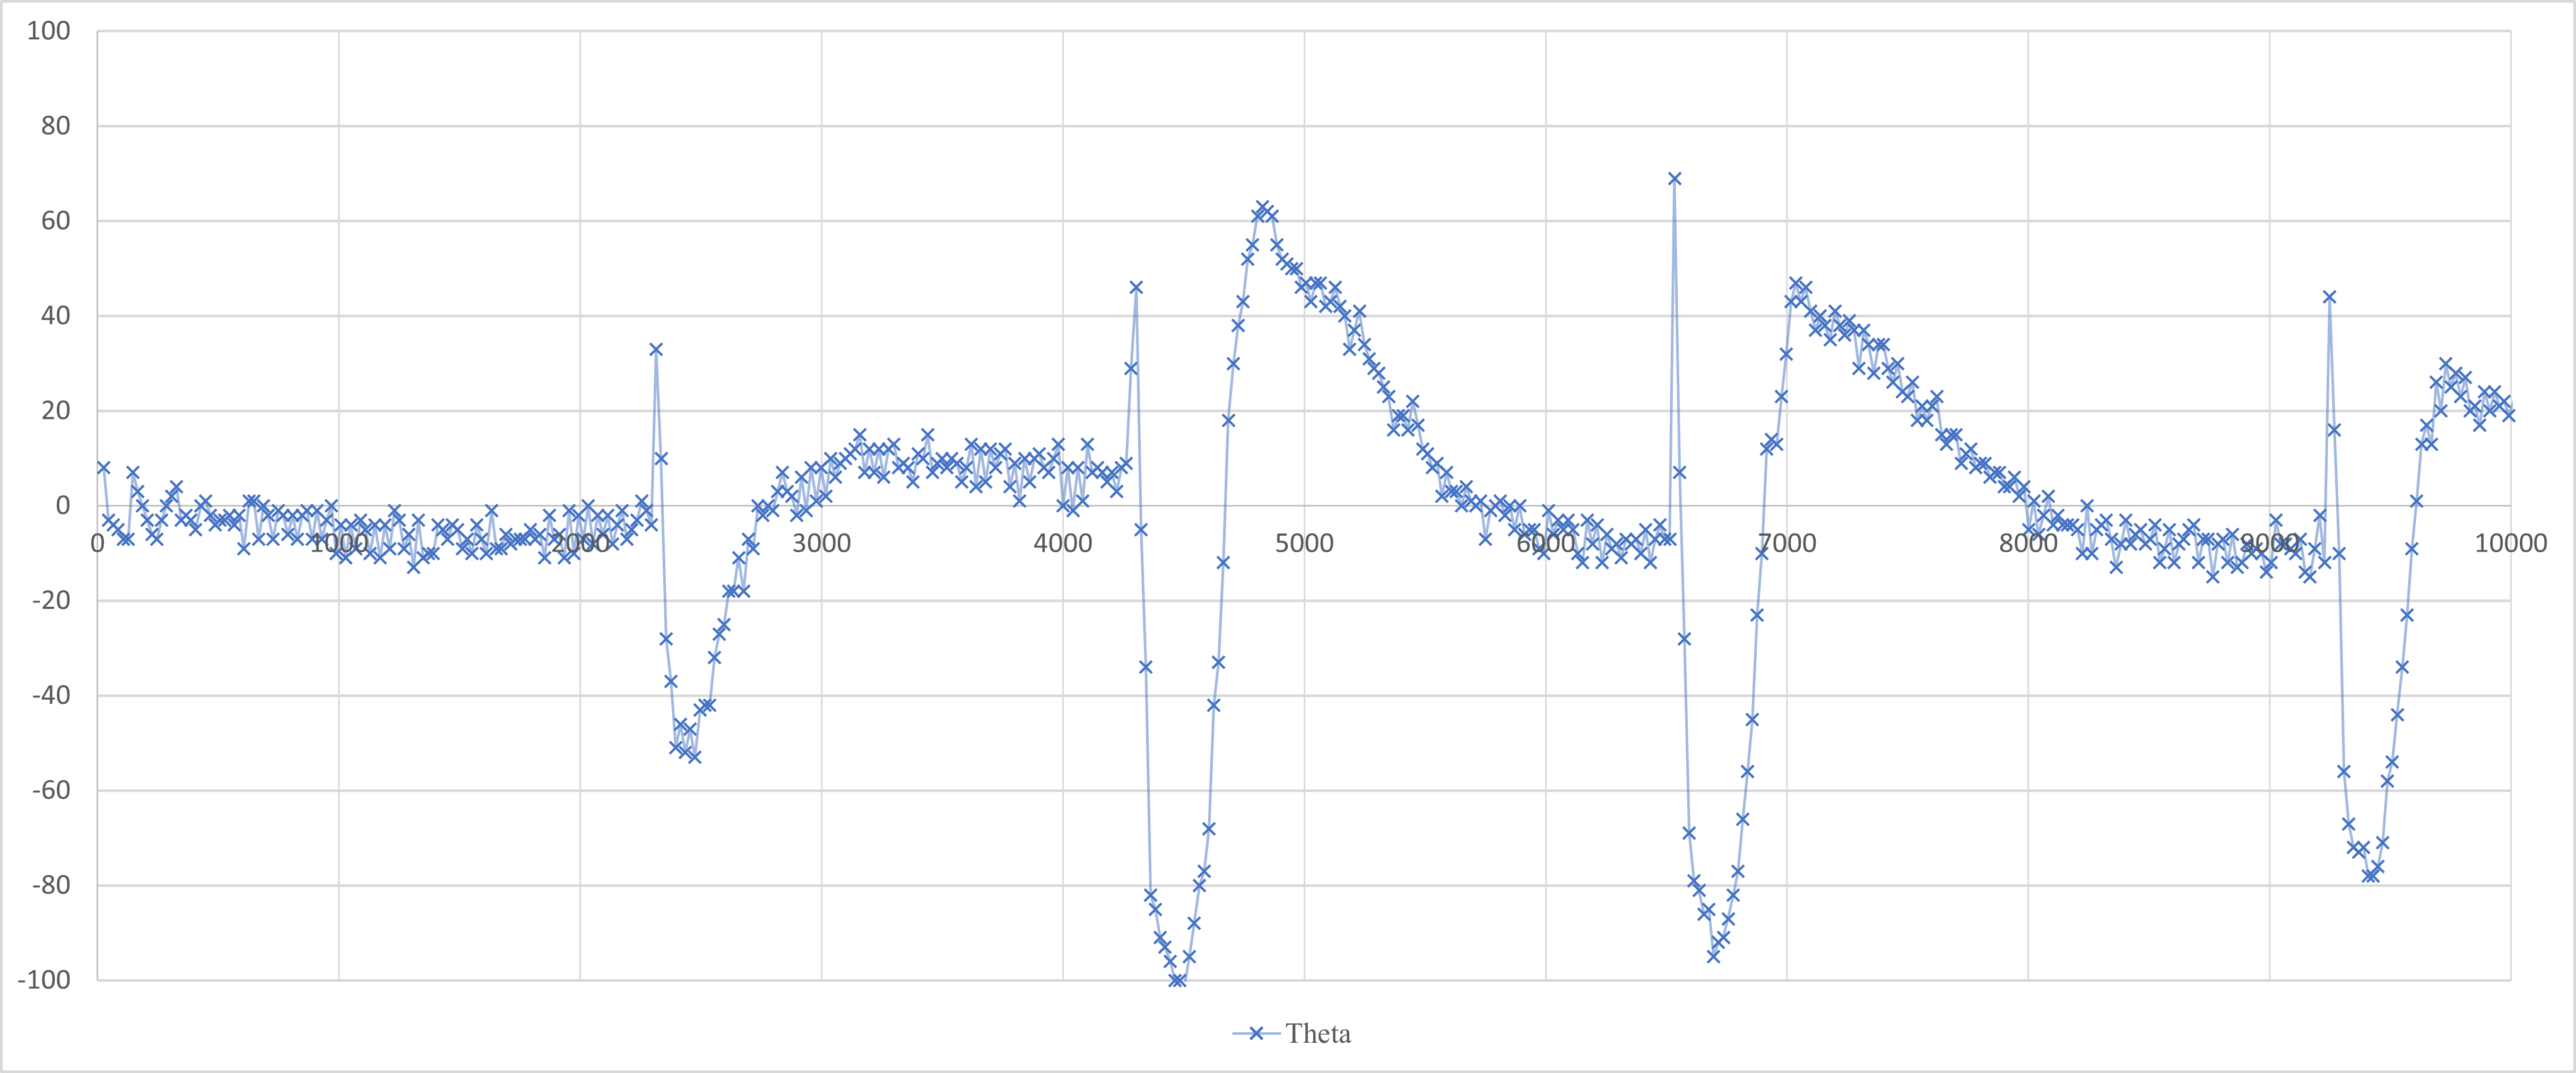
\includegraphics[width=\textwidth]{pictures/graphs/ThetaZN_00004.png}
    \caption{Plot of the drone on X-axis with calibrated values from Z-N method}
    \label{fig:Theta_ZN}
\end{figure}

From the testing, it was evident that overshoot was common, but it was chosen as a trade-off for the aggressive transient behaviour. Additionally, the interference from the finger results in a larger deviation in angle than it would in actual free flight circumstances.
\newpage

\subsubsection{Diagonal setup}

Testing in the string rig after tuning values in one-axis resulted in uncontrolled oscillations of the drone with no regards to the PID values. Due to that, the diagonal rig was set up and the code was changed accordingly.
The same procedure of axial testing was repeated for the diagonal rig and is described with figures \ref{fig:diagonal} and \ref{fig:ZN}.

\begin{figure}[h!]
    \centering
    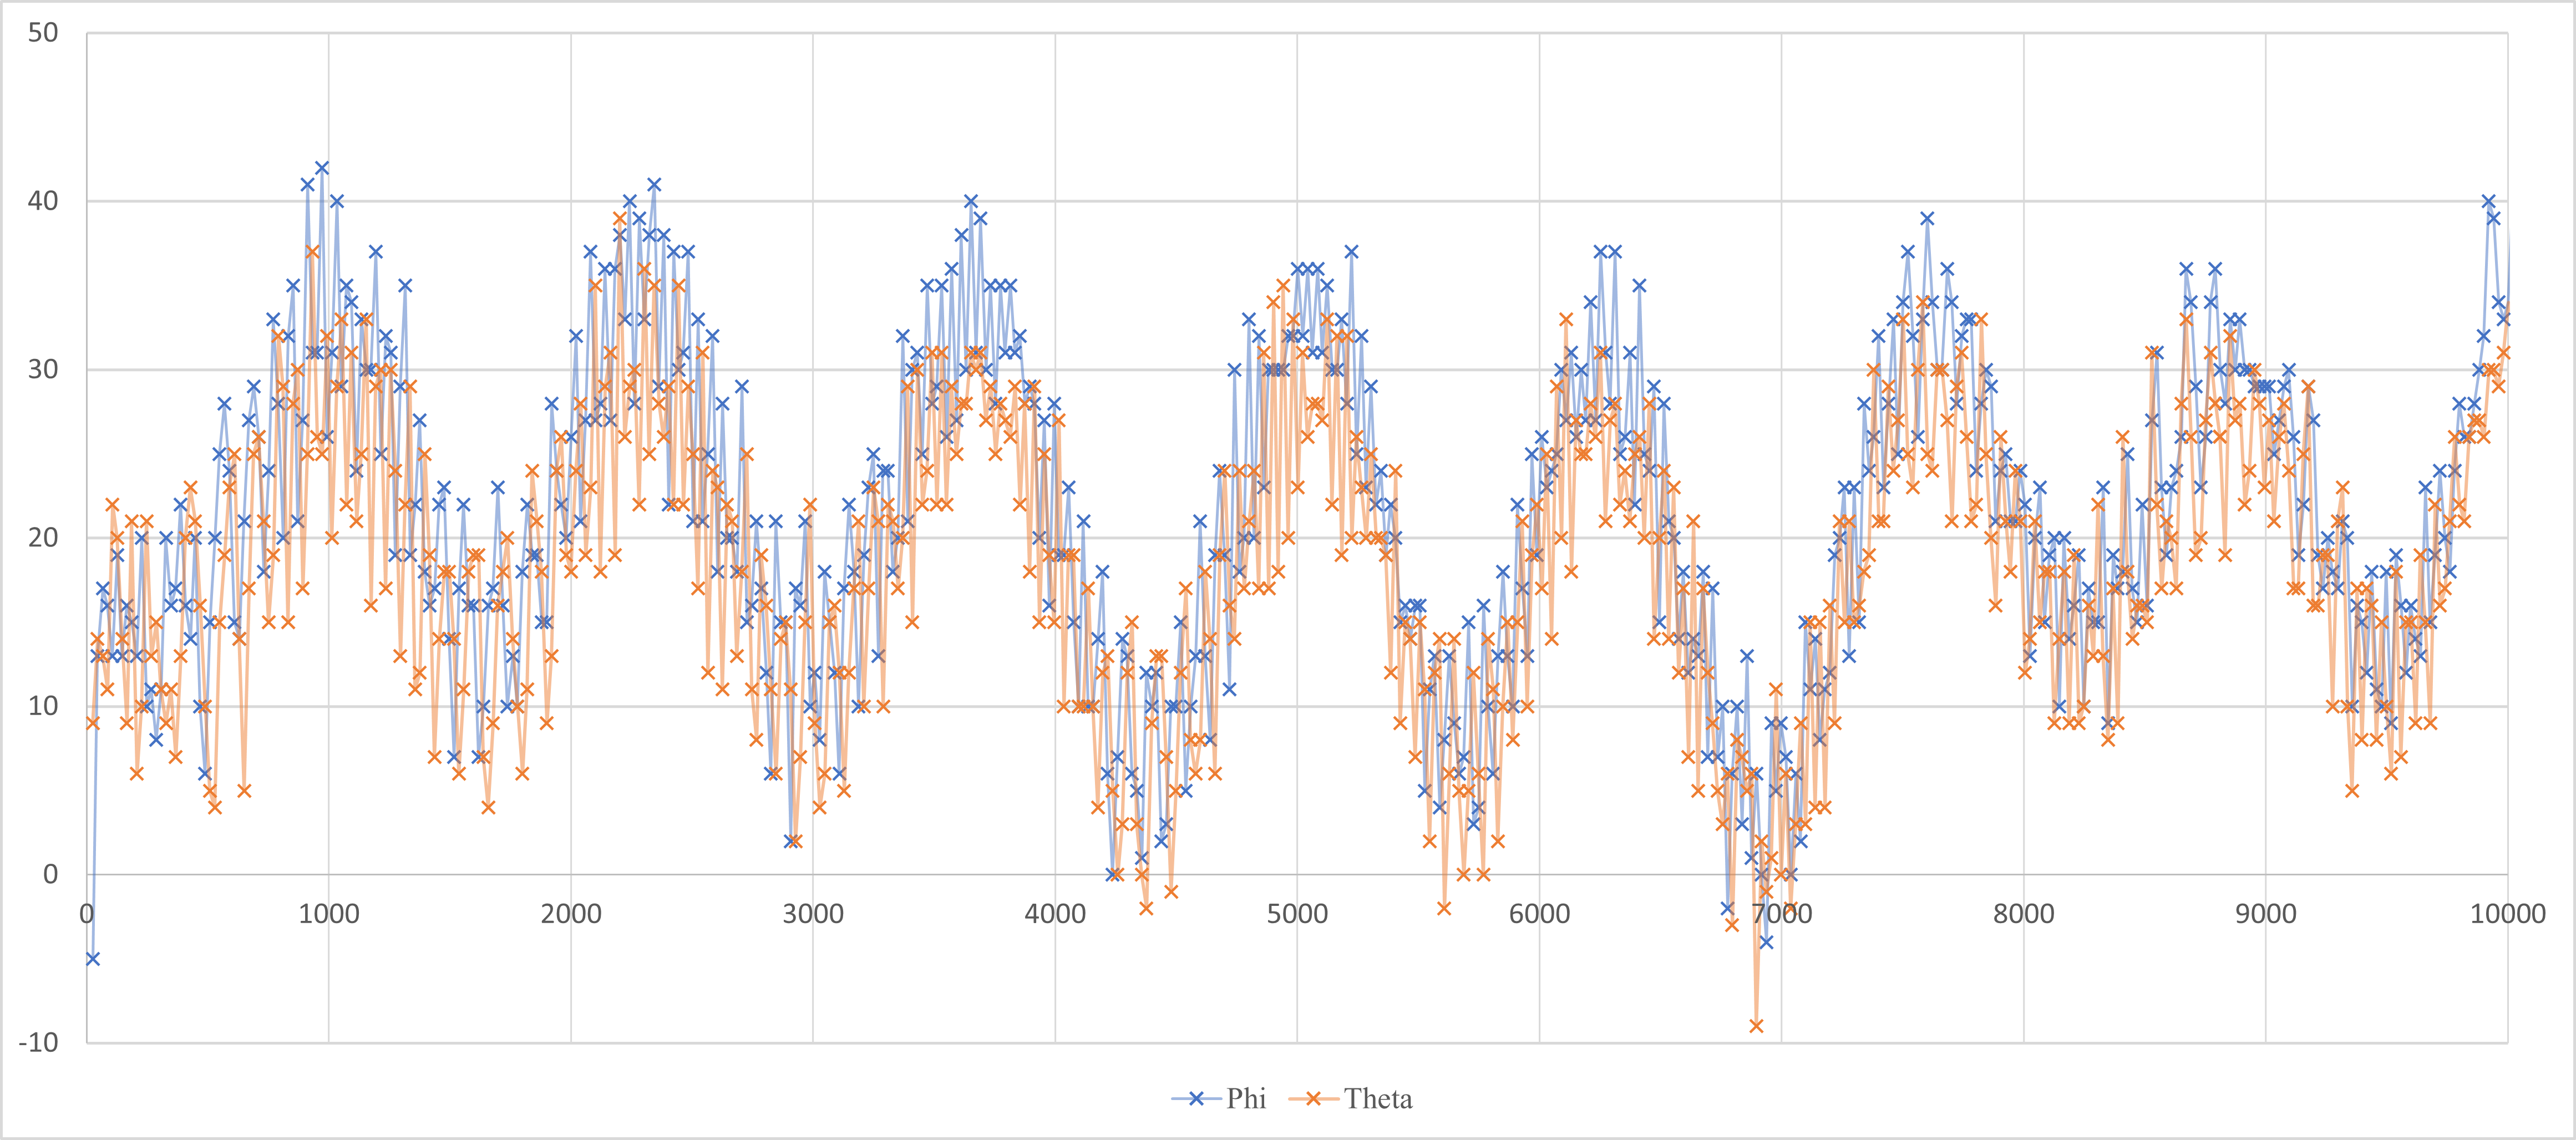
\includegraphics[width=\textwidth]{pictures/graphs/Diagonal_P0004.png}
    \caption{Plot of purely proportional control in diagonal setup for Z-N method}
    \label{fig:diagonal}
\end{figure}

\begin{figure}[h!]
    \centering
    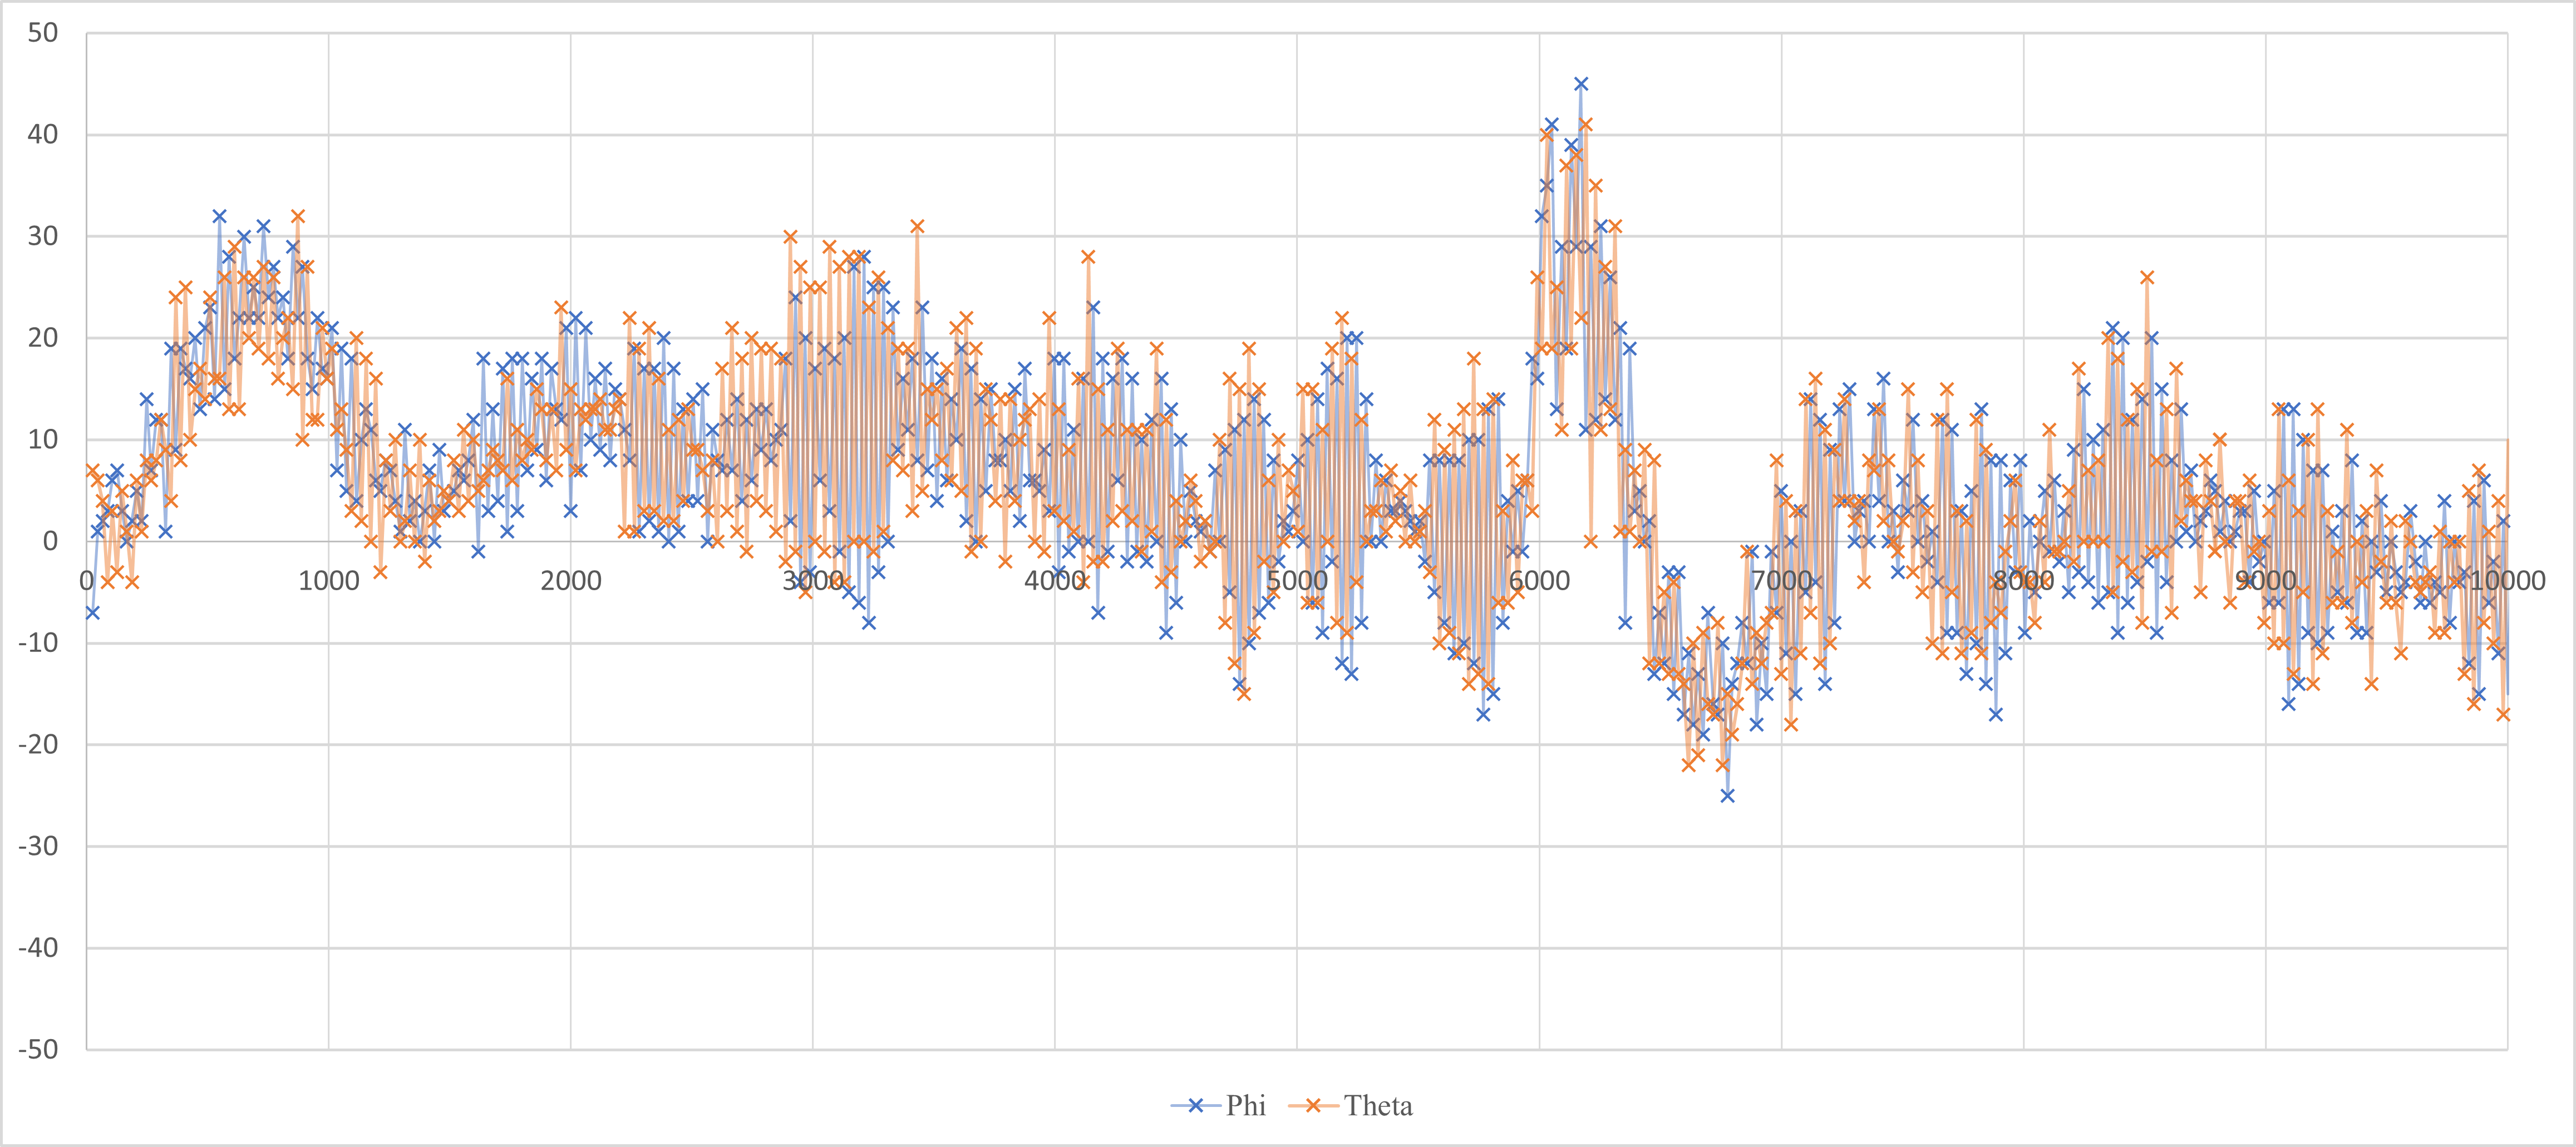
\includegraphics[width=\textwidth]{pictures/graphs/ZN.png}
    \caption{Plot of angles after using Z-N method from 'P' in figure \ref{fig:diagonal}}
    \label{fig:ZN}
\end{figure}

\newpage
\subsubsection{String setup}
The final testing rig was chosen to be the string rig (figure \ref{fig:string_rig}). A halo was attached to the top of the drone, so that the string attached to the drone would be put through, thus resulting in the strings not colliding with the propellers in different angles.

\begin{figure}[h]
    \centering
    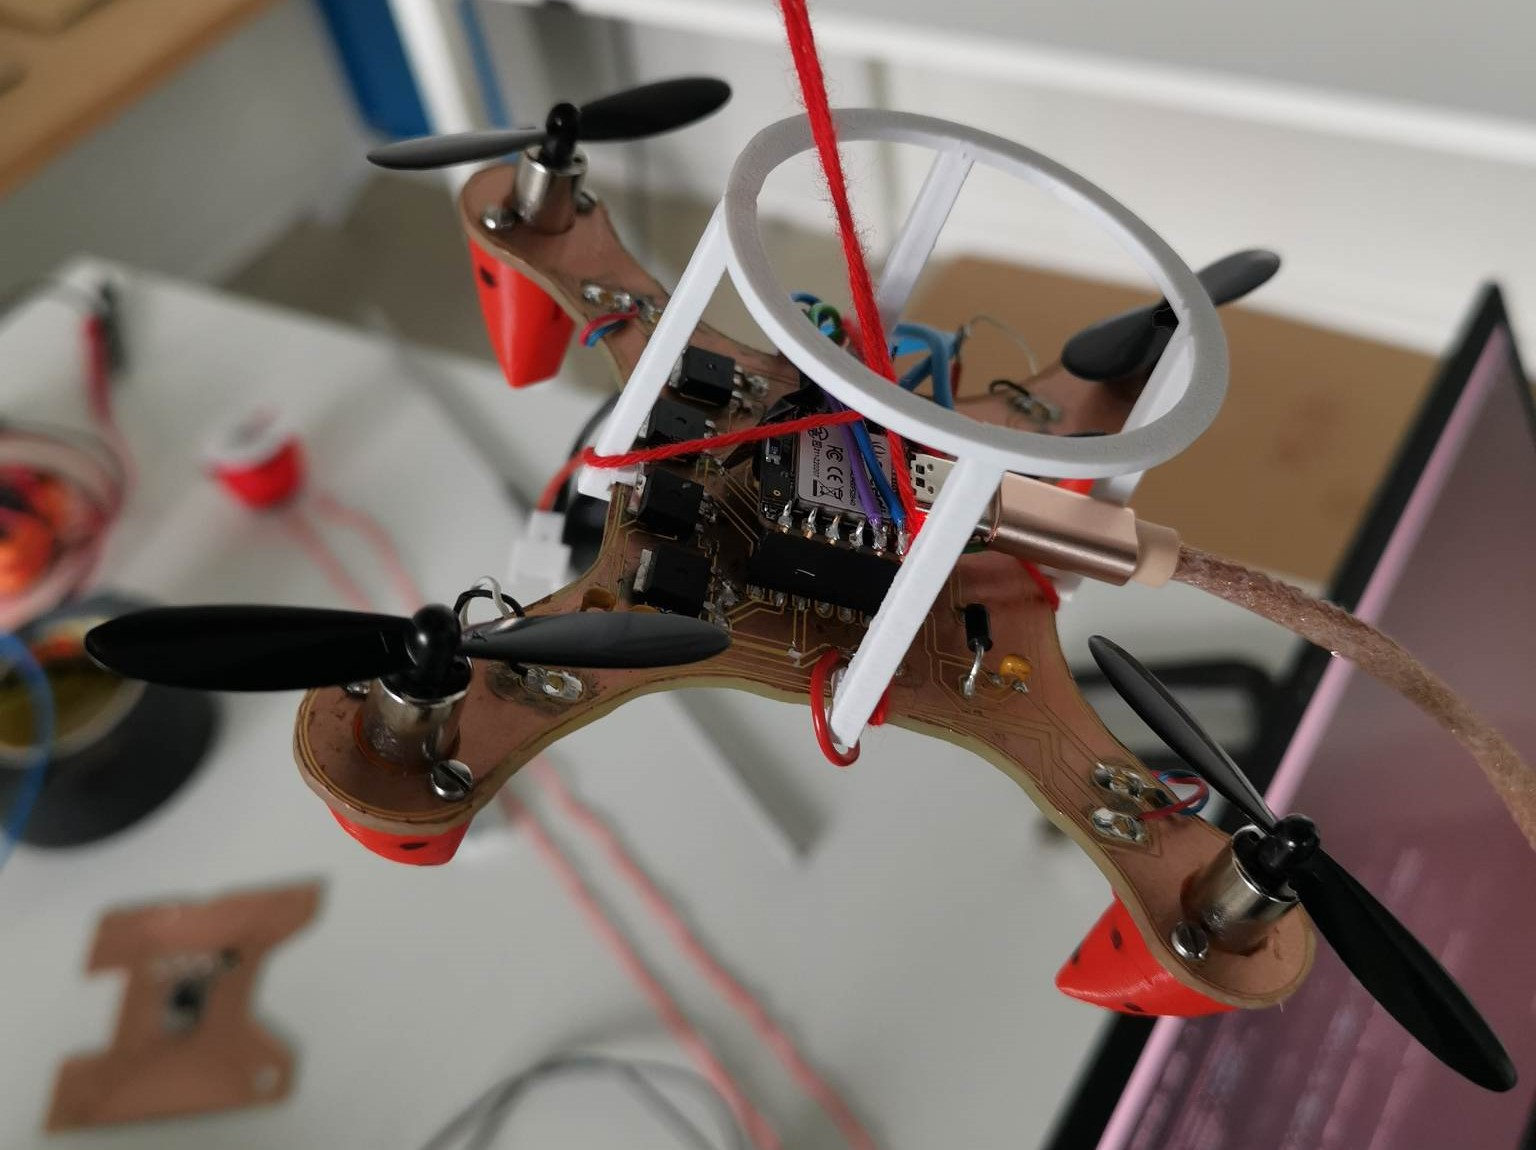
\includegraphics[width=\textwidth]{pictures/String_rig.jpg}
    \caption{String rig}
    \label{fig:string_rig}
\end{figure}

This provides the closest possible resemblance to flight that could achieved. It may adversely effect the flight characteristics, as the string pulls the drone to the center, which may result in tilt while flying away from the anchor point, but the other option was a gimbal, which introduced large friction.

The values from previous test runs were used at the start, but were found to be insufficient to compensate. Post testing, the ideal values were found to be 10 times the P and 5 times the D compared to the ones used in the diagonal rig. With these values $\phi$ was stable, however $\theta$ was oscillating between stability and instability, as it was initially stable, then became unstable, then became stable again. This was accounted for with higher PID constants for theta.

\begin{figure}[h!]
    \centering
    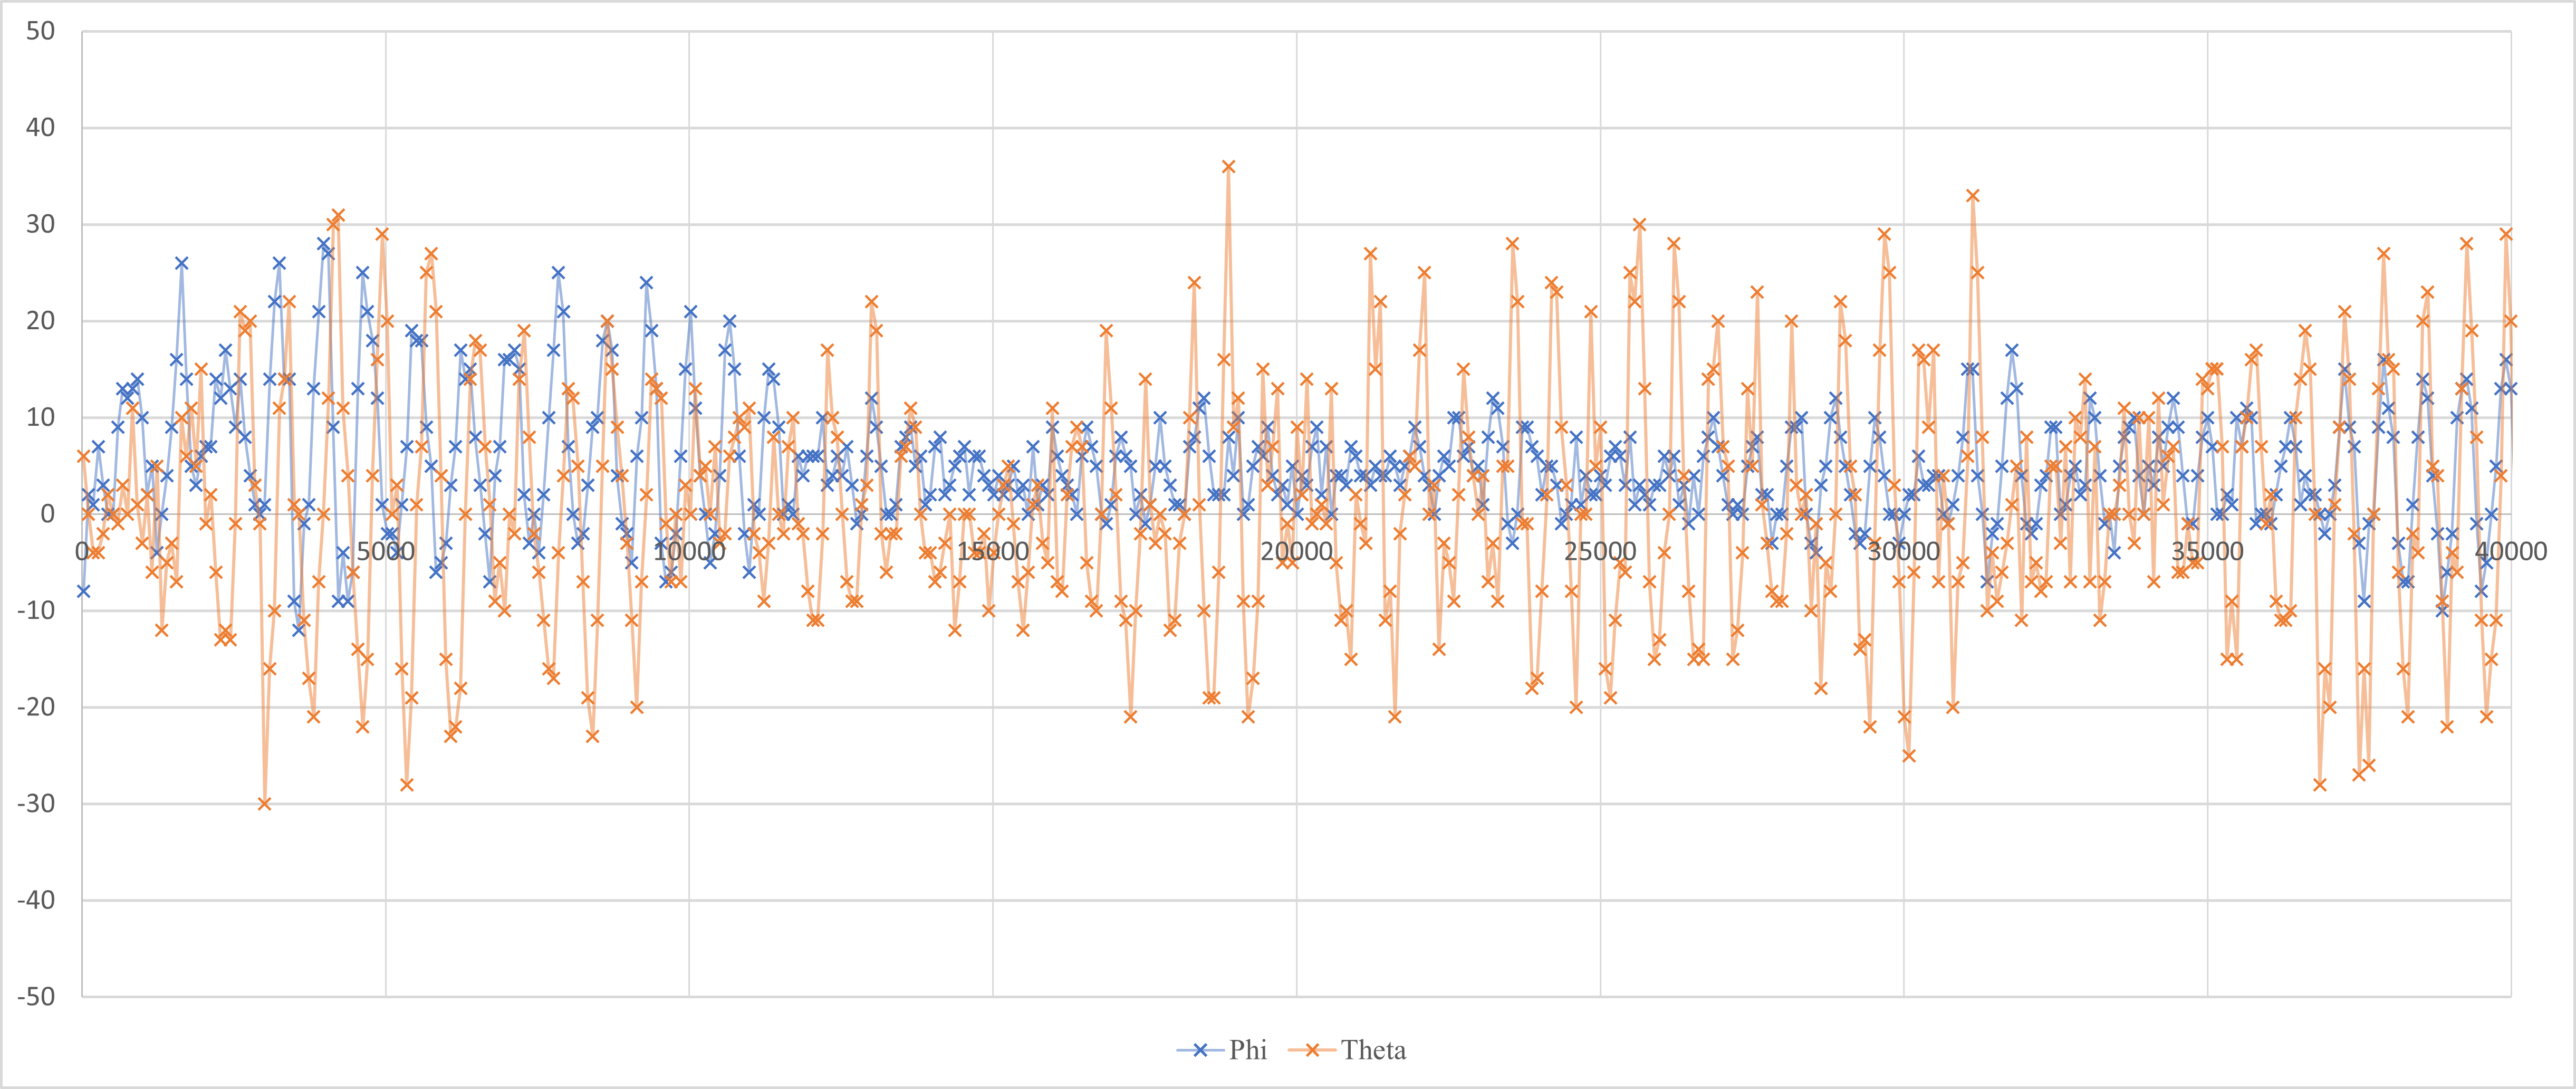
\includegraphics[width=\textwidth]{pictures/graphs/ZN10P5DT4The5.png}
    \caption{Plot of angles in string setup with calibrated PID values}
    \label{fig:ZN10P}
\end{figure}

\subsubsection{Conclusion of PID testing}

While independent flight was not achieved due to insufficient thrust, the PID system worked in a limited time frame. The instability in $\theta$ during string testing was nearly unaffected even with the 5x multiplier. This points to the possibility of the insufficient thrust affecting the authority of the PID control.
The other sources of instability could potentially be the differences between motors in different temperatures and RPMs or IMU deviation and drift.
